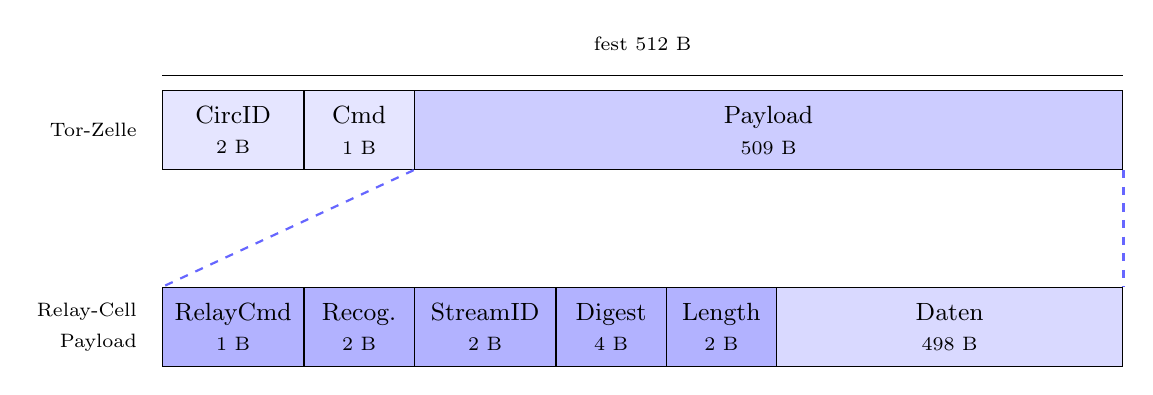
\begin{tikzpicture}[
    >=latex,
    every node/.style={font=\small},
    hdrbox/.style={
        draw, minimum height=10mm,
        align=center, fill=blue!10
    },
    plbox/.style={
        draw, minimum height=10mm,
        align=center, fill=blue!20
    },
    rhdrbox/.style={
        draw, minimum height=10mm,
        align=center, fill=blue!30
    },
    rdatabox/.style={
        draw, minimum height=10mm,
        align=center, fill=blue!15
    },
    lbl/.style={font=\scriptsize, anchor=east}
]

% ----------------------------------------------------------
% Obere Zeile: gesamte Tor-Zelle (512 B)
% Felder: CircID (2 B) | Command (1 B) | Payload (509 B)
% ----------------------------------------------------------
\node[lbl] at (-2mm, 5mm) {Tor-Zelle};

\node[hdrbox, minimum width=18mm] (h1) at (9mm,  5mm) {CircID\\\scriptsize 2 B};
\node[hdrbox, minimum width=14mm] (h2) at (25mm, 5mm) {Cmd\\\scriptsize 1 B};
\node[plbox,  minimum width=90mm] (pl) at (77mm, 5mm) {Payload\\\scriptsize 509 B};

% Hinweislinie oben: fest 512 B
\node[font=\scriptsize] at (61mm, 16mm) {fest 512 B};
\draw (0mm, 12mm) -- (122mm, 12mm);

% ----------------------------------------------------------
% Untere Zeile: Aufschluesselung der Relay-Cell-Payload (509 B)
% Felder: RelayCmd (1 B) | Recognized (2 B) | StreamID (2 B)
%       | Digest (4 B)   | Length (2 B)     | Daten (498 B)
% ----------------------------------------------------------
\node[lbl] at (-2mm, -18mm) {Relay-Cell};
\node[lbl] at (-2mm, -22mm) {Payload};

\node[rhdrbox,  minimum width=18mm] (r1) at (9mm,   -20mm) {RelayCmd\\\scriptsize 1 B};
\node[rhdrbox,  minimum width=14mm] (r2) at (25mm,  -20mm) {Recog.\\\scriptsize 2 B};
\node[rhdrbox,  minimum width=18mm] (r3) at (41mm,  -20mm) {StreamID\\\scriptsize 2 B};
\node[rhdrbox,  minimum width=14mm] (r4) at (57mm,  -20mm) {Digest\\\scriptsize 4 B};
\node[rhdrbox,  minimum width=14mm] (r5) at (71mm,  -20mm) {Length\\\scriptsize 2 B};
\node[rdatabox, minimum width=44mm] (r6) at (100mm, -20mm) {Daten\\\scriptsize 498 B};

% Zoom-in: gestrichelte Linien vom Payload in der oberen Zeile
% zu den Aussenkanten der unteren Aufschluesselung
\draw[thick, dashed, blue!60] (pl.south west) -- (r1.north west);
\draw[thick, dashed, blue!60] (pl.south east) -- (r6.north east);

\end{tikzpicture}
